\documentclass[tikz,border=10pt]{standalone}
\usepackage[T1]{fontenc}
\usepackage{lmodern}
\usepackage{amsmath}
\usepackage{graphicx}
\usetikzlibrary{arrows.meta,positioning,fit,calc,backgrounds,matrix}

\newcommand{\minirow}[3]{#1 & #2 & #3}
\newcommand{\maskedscoremat}{%
\begin{array}{c@{\;}c}
& \begin{array}{ccc} \mathbf{k}_1 & \mathbf{k}_2 & \mathbf{k}_3 \end{array}\\[-1mm]
\begin{array}{c} \mathbf{q}_1\\[1.8mm] \mathbf{q}_2\\[1.8mm] \mathbf{q}_3 \end{array}
&
\begin{bmatrix}
s_{11} & s_{12} & s_{13}\\
-\infty & s_{22} & s_{23}\\
-\infty & -\infty & s_{33}
\end{bmatrix}
\end{array}}
\newcommand{\alphamat}{\begin{bmatrix}
 \alpha_{11} & \alpha_{12} & \alpha_{13}\\
 0 & \alpha_{22} & \alpha_{23}\\
 0 & 0 & \alpha_{33}
\end{bmatrix}}

\begin{document}
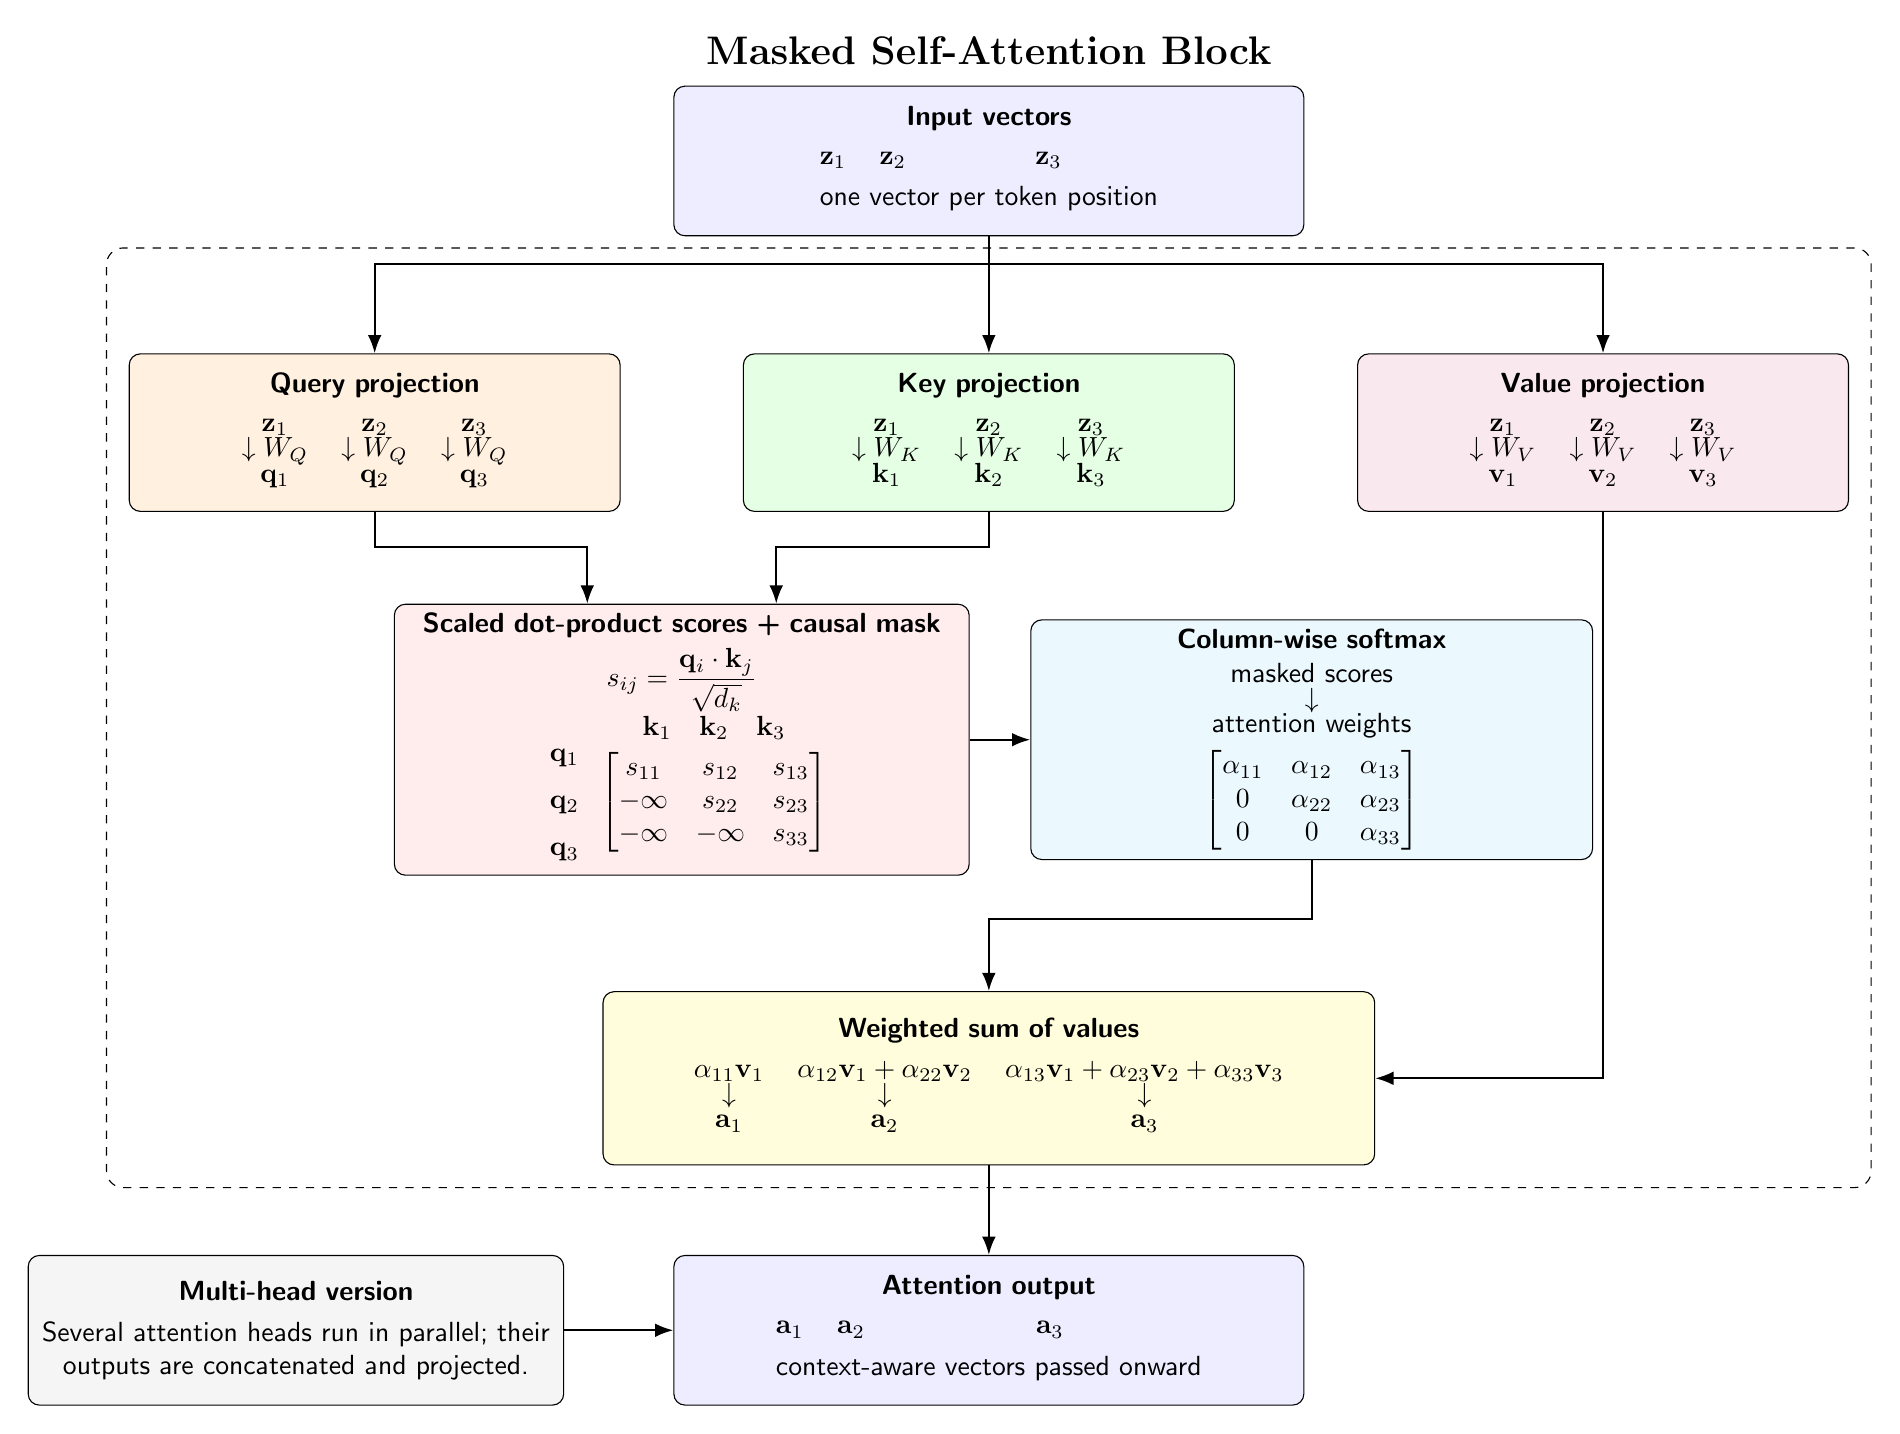
\begin{tikzpicture}[
    font=\sffamily,
    >=Latex,
    arrow/.style={->, thick},
    box/.style={draw, rounded corners=4pt, align=center, fill=blue!7,
        minimum width=8.0cm, text width=7.75cm, minimum height=1.9cm},
    smallbox/.style={draw, rounded corners=4pt, align=center, fill=blue!7,
        minimum width=6.8cm, text width=6.55cm, minimum height=1.9cm},
    qbox/.style={draw, rounded corners=4pt, align=center, fill=orange!12,
        minimum width=6.2cm, text width=6.0cm, minimum height=2.0cm},
    kbox/.style={draw, rounded corners=4pt, align=center, fill=green!10,
        minimum width=6.2cm, text width=6.0cm, minimum height=2.0cm},
    vbox/.style={draw, rounded corners=4pt, align=center, fill=purple!9,
        minimum width=6.2cm, text width=6.0cm, minimum height=2.0cm},
    scorebox/.style={draw, rounded corners=4pt, align=center, fill=red!7,
        minimum width=7.3cm, text width=7.05cm, minimum height=3.25cm},
    softbox/.style={draw, rounded corners=4pt, align=center, fill=cyan!8,
        minimum width=7.1cm, text width=6.9cm, minimum height=2.5cm},
    outbox/.style={draw, rounded corners=4pt, align=center, fill=yellow!14,
        minimum width=7.1cm, text width=6.9cm, minimum height=2.2cm},
    dashedbox/.style={draw, dashed, rounded corners=6pt, inner sep=8pt}
]

% Title
\node[font=\bfseries\Large] (title) at (7.8,2.0) {Masked Self-Attention Block};

% Input
\node[box] (input) at (7.8,0.6) {\textbf{Input vectors}\\[1mm]
\begin{tabular}{ccc}
$\mathbf{z}_1$ & $\mathbf{z}_2$ & $\mathbf{z}_3$\\[1mm]
\multicolumn{3}{c}{one vector per token position}
\end{tabular}};

% Q K V projections
\node[qbox] (qproj) at (0,-2.85) {\textbf{Query projection}\\[1mm]
\begin{tabular}{ccc}
$\mathbf{z}_1$ & $\mathbf{z}_2$ & $\mathbf{z}_3$\\[-1mm]
$\downarrow W_Q$ & $\downarrow W_Q$ & $\downarrow W_Q$\\[-1mm]
$\mathbf{q}_1$ & $\mathbf{q}_2$ & $\mathbf{q}_3$
\end{tabular}};

\node[kbox] (kproj) at (7.8,-2.85) {\textbf{Key projection}\\[1mm]
\begin{tabular}{ccc}
$\mathbf{z}_1$ & $\mathbf{z}_2$ & $\mathbf{z}_3$\\[-1mm]
$\downarrow W_K$ & $\downarrow W_K$ & $\downarrow W_K$\\[-1mm]
$\mathbf{k}_1$ & $\mathbf{k}_2$ & $\mathbf{k}_3$
\end{tabular}};

\node[vbox] (vproj) at (15.6,-2.85) {\textbf{Value projection}\\[1mm]
\begin{tabular}{ccc}
$\mathbf{z}_1$ & $\mathbf{z}_2$ & $\mathbf{z}_3$\\[-1mm]
$\downarrow W_V$ & $\downarrow W_V$ & $\downarrow W_V$\\[-1mm]
$\mathbf{v}_1$ & $\mathbf{v}_2$ & $\mathbf{v}_3$
\end{tabular}};

% Scores
\node[scorebox] (scores) at (3.9,-6.75) {\textbf{Scaled dot-product scores + causal mask}\\[1mm]
\begin{tabular}{c}
$s_{ij}=\dfrac{\mathbf{q}_i\cdot \mathbf{k}_j}{\sqrt{d_k}}$\\[1mm]
$\maskedscoremat$
\end{tabular}};

% Softmax
\node[softbox] (softmax) at (11.9,-6.75) {\textbf{Column-wise softmax}\\[1mm]
\begin{tabular}{c}
masked scores\\[-1mm]
$\downarrow$\\[-1mm]
attention weights\\[1mm]
$\alphamat$
\end{tabular}};

% Weighted values
\node[outbox, minimum width=9.8cm, text width=9.55cm] (weighted) at (7.8,-11.05) {\textbf{Weighted sum of values}\\[1mm]
\begin{tabular}{ccc}
$\alpha_{11}\mathbf{v}_1$ & $\alpha_{12}\mathbf{v}_1+\alpha_{22}\mathbf{v}_2$ & $\alpha_{13}\mathbf{v}_1+\alpha_{23}\mathbf{v}_2+\alpha_{33}\mathbf{v}_3$\\[-1mm]
$\downarrow$ & $\downarrow$ & $\downarrow$\\[-1mm]
$\mathbf{a}_1$ & $\mathbf{a}_2$ & $\mathbf{a}_3$
\end{tabular}};

% Output
\node[box] (output) at (7.8,-14.25) {\textbf{Attention output}\\[1mm]
\begin{tabular}{ccc}
$\mathbf{a}_1$ & $\mathbf{a}_2$ & $\mathbf{a}_3$\\[1mm]
\multicolumn{3}{c}{context-aware vectors passed onward}
\end{tabular}};

% Optional multi-head note
\node[smallbox, fill=gray!8] (multihead) at (-1.0,-14.25) {\textbf{Multi-head version}\\[1mm]
Several attention heads run in parallel; their outputs are concatenated and projected.};

% Arrows
\draw[arrow] (input.south) -- ++(0,-0.35) -| (qproj.north);
\draw[arrow] (input.south) -- (kproj.north);
\draw[arrow] (input.south) -- ++(0,-0.35) -| (vproj.north);

\draw[arrow] (qproj.south) -- ++(0,-0.45) -| ([xshift=-1.2cm]scores.north);
\draw[arrow] (kproj.south) -- ++(0,-0.45) -| ([xshift=1.2cm]scores.north);

\draw[arrow] (scores.east) -- (softmax.west);

\coordinate (softmaxToWeightedA) at ($(softmax.south)+(0,-0.75)$);
\coordinate (softmaxToWeightedB) at ($(weighted.north)+(4.1,0.75)$);
\draw[arrow] (softmax.south) -- (softmaxToWeightedA) -| (weighted.north);

\coordinate (valueToWeightedA) at ($(vproj.south)+(0,-6.95)$);
\coordinate (valueToWeightedB) at ($(weighted.east)+(0.9,0)$);
\draw[arrow] (vproj.south) -- (valueToWeightedA) |- (weighted.east);

\draw[arrow] (weighted.south) -- (output.north);

\draw[arrow] (multihead.east) -- (output.west);

\begin{pgfonlayer}{background}

% Invisible helper node: extends the dashed box upward so the input arrow branches inside it.
\node[inner sep=0pt, minimum width=0.1cm, minimum height=0.1cm] (branchfit) at ($(qproj.north)!0.5!(vproj.north)+(0,1.00)$) {};

\node[dashedbox, fit=(branchfit)(qproj)(kproj)(vproj)(scores)(softmax)(weighted)] (attentionfit) {};
\end{pgfonlayer}

\end{tikzpicture}
\end{document}
